%*****************************************************************************************
%*********************************** First Chapter ***************************************
%*****************************************************************************************

\chapter{Introduction}

\graphicspath{{Chapter1/Figures/}}

Semiconducting behaviour was first reported by Michael Faraday, who noted in 1839 that the conductivity of silver selenide increased with temperature, opposite to what is expected for a metal \cite{Faraday2012}. Photovoltaic behaviour was observed in silver chloride coated platinum electrodes, where illumination with sunlight caused an increase in the induced voltage \cite{Becquerel1839}, and the first photovoltaic cell used 30\,$\mu$m thick selenium film with thin gold leaf contacts, which produced efficiency <1\% \cite{Fritts1883}. Photoconductivity was first reported in selenium bars as a result of exposure to sunlight \cite{Smith1873, Adams1876}, while electroluminescent behaviour was first shown in SiC \cite{Round1907}. Simple principles such as these underpin the electronic devices we use today, yet it was not until Alan Wilson's work on band theory in 1931 that such behaviour could be understood and explained \cite{Wilson1931}. 

Throughout the 20th Century research was focused on using semiconductors for devices, from the developments of rectifiers and diodes in the early part of the century to the first Ge transistor built at Bell Laboratories in 1946 [Fig.\,\ref{1Fig1}(a)]. Since then, much work has been undertaken to refine and improve these devices to create more sophisticated designs used today. However device efficiency still hinges on the quality of the semiconducting materials used, and the ability to control impurities and dopants in the crystal. While the earliest devices used materials such as lead selenide, Si and Ge are currently commonly used.

Si is most widely used in the semiconductor industry due to its abundance in the Earth's crust, low unit cost and simple and well-developed processing techniques. Its high band gap gives it thermal stability, allowing it to be used at high operating temperatures. Si is also highly mechanically stable with high electron mobility, and the native insulating oxide layer can be useful in electronics. Although Ge has higher conductivity than Si, its lower band gap gives devices more temperature sensitivity. although alloys of Si and Ge may be used to combine the properties of both materials. Poor emission properties of Si as a result of its indirect band gap is one of the main disadvantages of the material, however GaAs has a large direct band gap and high electron mobility, which means it can be used in high speed devices. Other alloys, for example between Group III-V or II-VI elements, can be produced to provide specified optoelectronic properties, or combined to make lower dimension structures that can produce other desirable properties.
\begin{figure}[h!]
\centering
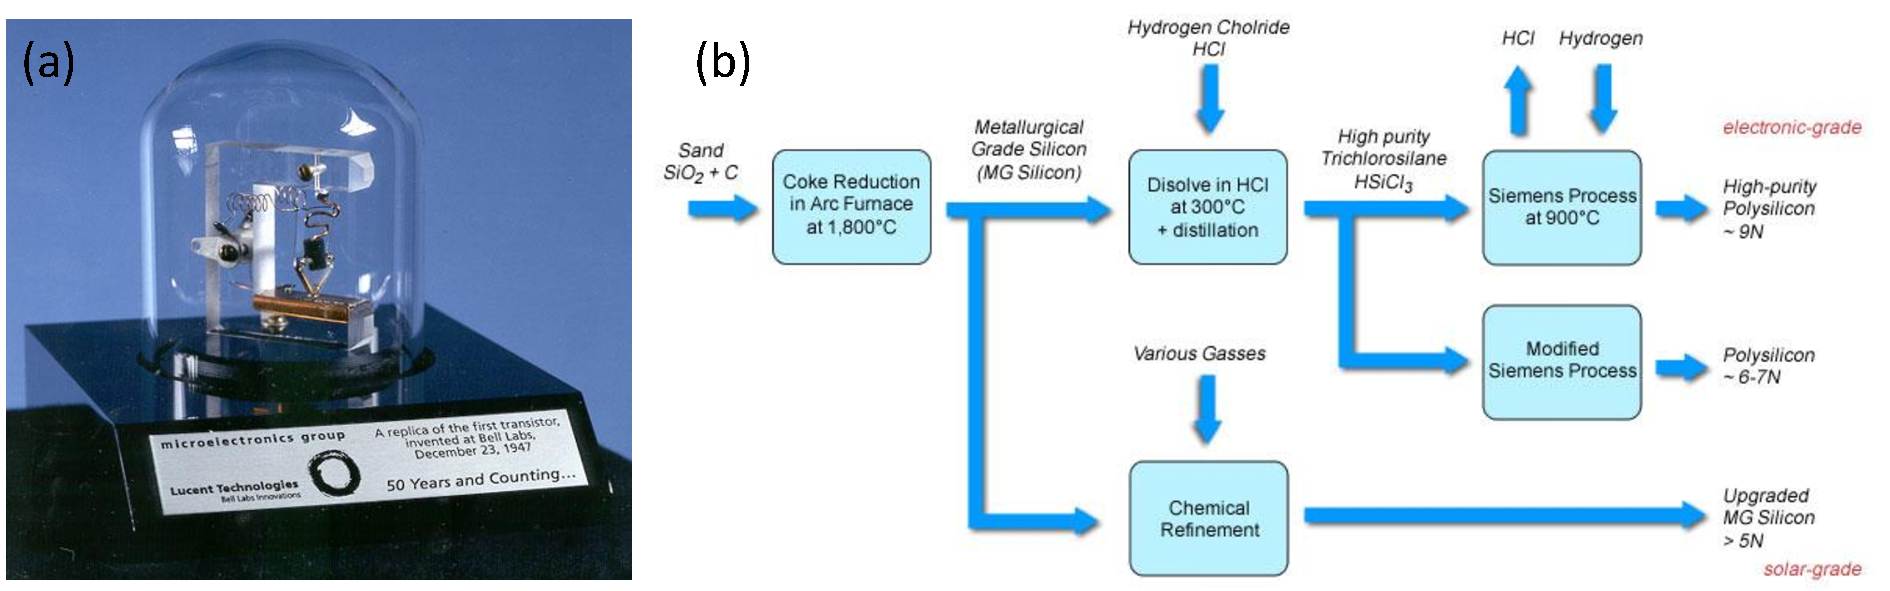
\includegraphics[width=\textwidth]{Fig1}
\caption{(a) Replica of first transistor built in 1946. Reproduced from Ref.\,\cite{Transistor}. (b) Process required to produce device-grade silicon from starting materials. Reproduced from Ref.\,\cite{Silicon}.}
\label{1Fig1}
\end{figure}

Despite the high stability and carrier mobility shown by inorganic semiconductors, one major disadvantage is with the processing of such materials. Although Si processing is well-developed, creation of device-grade material still requires many purification steps [Fig.\,\ref{1Fig1}(b)]. Alloys are often produced using vapour or electron-beam deposition, where deposition parameters must be strictly controlled. Layer-by-layer growth can be used for the best quality samples, however such processes are costly and time consuming. Current advances in technology require flexible, lightweight and more easily processable semiconductors, as well as control over the behaviour of carriers. 

\begin{figure}[h!]
\centering
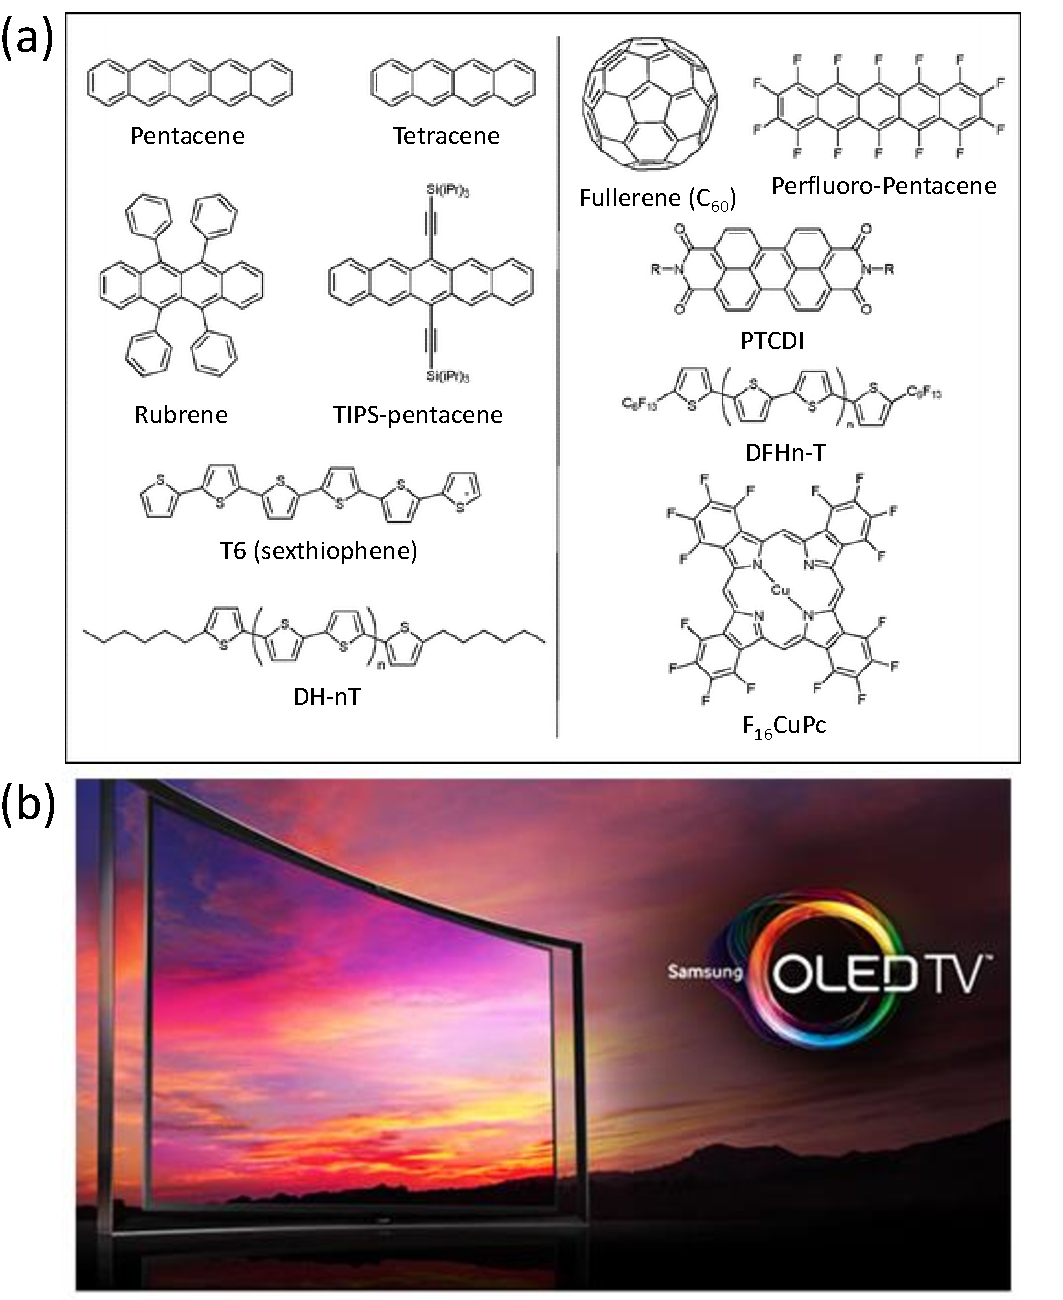
\includegraphics[width=0.8\textwidth]{Fig2}
\caption{(a) Common organic semiconductors, with p-type materials on the left and n-type on the right. Modified from Ref.\,\cite{Miozzo2010}. (b) Samsung curved smart OLED TV. Reproduced from Ref.\,\cite{Samsung}.}
\label{1Fig2}
\end{figure}
Although conduction was noted in a mix of aniline and sulphiric acid by Henry Letherby in 1862, research on organic seminconductors began in earnest in the latter half of the 20th Century. Polycyclic aromatic compounds were found to form semiconducting charge transfer complexes with halogens \cite{Naarmann2002}, and since then much work has been done on developing new molecules and polymers, driven by the relative ease with which such molecules can be synthesised. Organic semiconductors generally consist of conjugated molecules, whose overlapping $\pi$ orbitals allow charge transport within the molecule [Fig.\,\ref{1Fig2}(a)]. Given the low production cost, work has been undertaken to produce devices made of organic semiconductors, notably organic photovoltaics and thin film transistors. The organic light emitting diode (OLED) is probably the most technologically mature application of organic electronics, as OLEDs are currently used mobile phone displays and TVs, and offer better efficiency and brightness than other display technologies [Fig.\,\ref{1Fig2}(b)]. However problems exist with the manufacture of such devices as mass production is not currently optimised for the organic electronic market. More fundamentally, organic semiconductors are less thermally, optically and electrically stable than their inorganic counterparts, leading to lower device lifespan. Charge mobility is also lower as hopping between adjacent molecules is required, and lower crystallinity leads to increased scattering at grain boundaries. 

A new class of hybrid materials has emerged in the last 25 years. Metal halide-based organic-inorganic perovskite semiconductors combine the stability of the inorganic semiconductors with the processability of organic semiconductors. A variety self-assembling of inorganic frameworks can form and accommodate excited charge carriers, while organic moeities can be used to further modify material properties \cite{Cheng2010, Ishihara1990, Mitzi2001, Mitzi2001c, Nagami1996, Pradeesh2010, Pradeesh2009a Lee2012, Heo2013, Liu2013, Hao2014}. Such perovskites can be incorporated into nanostructures to form new mixed states with novel properties \cite{Fujita1998, Fujita1999, Fujita2000, Ishi-Hayase2003, Brehier2006, Lanty2008, Pradeesh2009b, Sumioka2001}.

This thesis explores the optical properties of 2D lead iodide-based perovskites, particularly the interactions between perovskite excitons and collective electron oscillations called surface plasmons. I will first introduce the theory of excitons and review the research on lead iodide perovskites, before exploring the optical properties of noble metal nanostructures. In Chapter 4 I will describe the fabrication of perovskite thin films via spin coating, then study the optical properties of ultra-thin perovskite samples produced via exfoliation in Chapter 5. In Chapter 6 I will explore exciton-localised surface plasmon interactions in perovskite-coated nano-island structures. Finally in Chapter 7 I will examine the coupling between excitons and surface plasmon polaritons in perovskite-coated plasmonic gratings.